\section{Management Summary}
\subsection*{Ausgangslage}
OpenStreetMap (OSM) ist ein Wikipedia-artiges Projekt mit einer Webkarte ähnlich wie Google Maps. OSM bietet unter anderem freie Geodaten, die auch für Fussgängernavigation genutzt werden können. Dabei müssen die bestehenden Fussgängerstreifen in die Routenplanung einbezogen werden, um eine Überquerung der Strassen zu ermöglichen. Gemäss heutigem Stand sind noch lange nicht alle Fussgängerstreifen in OSM erfasst, was die Fussgängernavigation erschwert.

Dieses Projekt ist der Versuch einer automatischen Erkennung von Fussgängerstreifen auf Orthofotos (Satellitenbilder). Da das maschinelle Erfassen von Daten in OSM nicht erlaubt ist, können die gefundenen Koordinaten in ein Crowdsourcing-System wie zum Beispiel MapRoulette eingespeist werden. In diesem bewerten Nutzer, ob die eingefügten Daten korrekt sind oder nicht.

\subsection*{Vorgehen}
\begin{figure}[H]
	\centering
	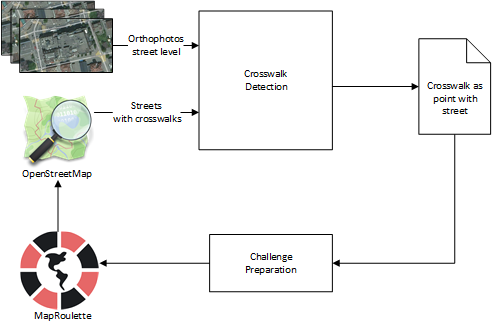
\includegraphics[width=410pt]{images/management_summary_1.png}
	\caption[Management Summery Überblick]{Überblick über den Datenfluss zur Erkennung und Erfassung von Fussgängerstreifen in OpenStreetMap.}
\end{figure}
\medskip
Die Arbeit begann mit der Evaluation eines passenden Bilderkennungsalgorithmus. Dabei wurden diverse Algorithmen zur Klassifikation der Bilder geprüft, vom Haar Feature-based Cascade Classifier über Fast Fourier Transform bis zu Neuronalen Netzen. Ein neuronales Netz, genauer ein Convolutional Neural Network, brachte die besten Resultate.

Weiter mussten Orthofotos, wie auch Informationen zu Strassenachsen und die Koordinaten der schon in OSM erfassten Fussgängerstreifen beschafft werden. Dabei konnte auf Bing Maps und die OSM-Programmierschnittstelle von MapQuest zurückgegriffen werden.

Da die Bilderkennung ein sehr rechenintensiver Prozess ist, musste der Erkennungsprozess parallelisiert werden. Mit Hilfe eines Docker Images und einem Queueing System konnte die Erkennung auf verschiedene Maschinen verteilt und der Erkennungsaufwand auf mehrere Tage beschränkt werden. Ohne diese Parallelisierung hätten Wartezeiten von mehreren Wochen in Kauf genommen werden müssen.


\subsection*{Ergebnisse}
Aus diesem Projekt entstand eine Applikation für die automatische Erkennung von Fussgängerstreifen. Diese bezieht in einem angegebenen Bereich, wie beschrieben, automatisch die entsprechenden Orthofotos und Strasseninformationen und extrahiert daraus die Koordinaten der Fussgängerstreifen. Die Koordinaten werden in einer JSON-Datei abgelegt und können in eine MapRoulette Challenge umgewandelt werden. 
\\
\begin{figure}[H]
	\centering
	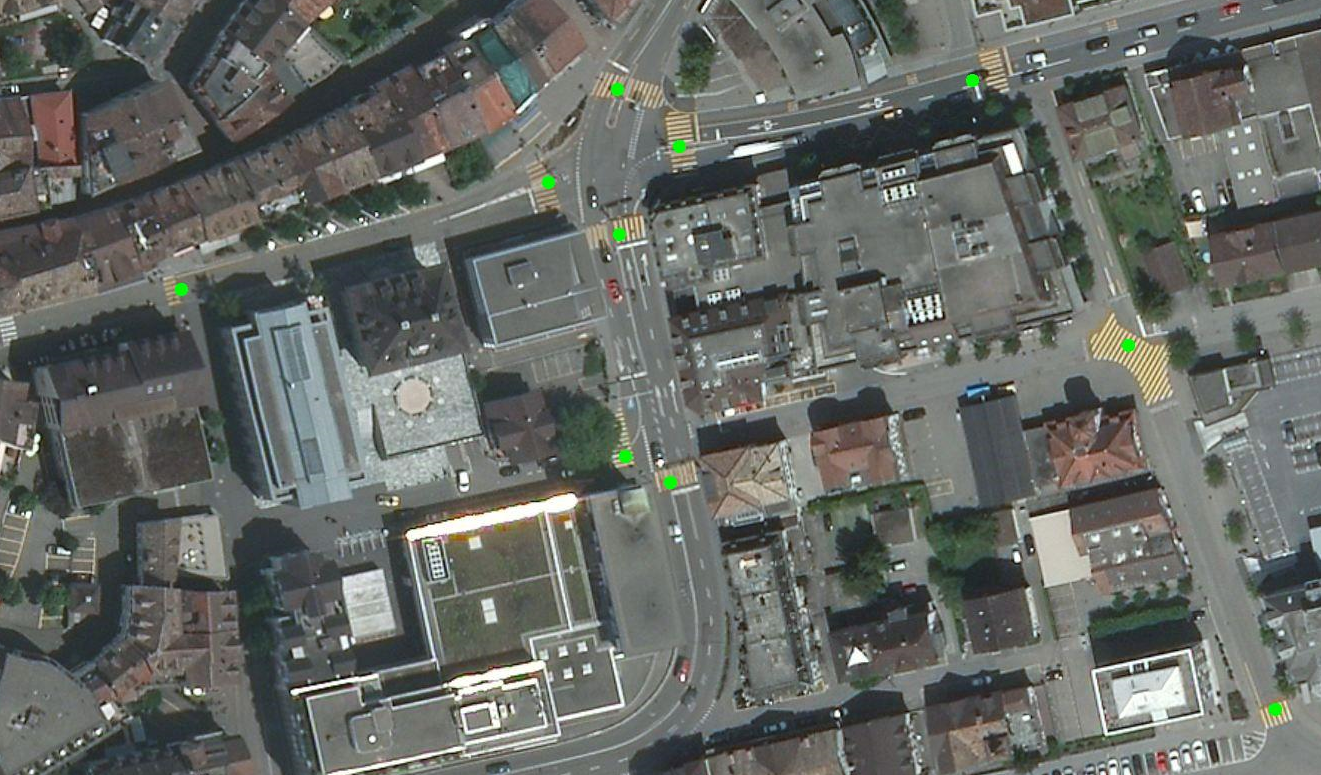
\includegraphics[width=\textwidth -10mm]{images/boxsave_rappi.png}
	\caption[Überblick]{Rapperswil Innenstadt - Gefundene Fussgängerstreifen sind mit einem grünen Punkt markiert.}
\end{figure}
\medskip
Die Applikation erkannte mehr als 80\% aller gelben Fussgängerstreifen mit einer Fehlerrate von weniger als 10\%. Die Koordinaten der Fussgängerstreifen im Raum der Kantone Zürich und Zug konnten an MapRoulette zur Einpflege in OSM übergeben werden.
\\
\begin{figure}[H]
	\centering
	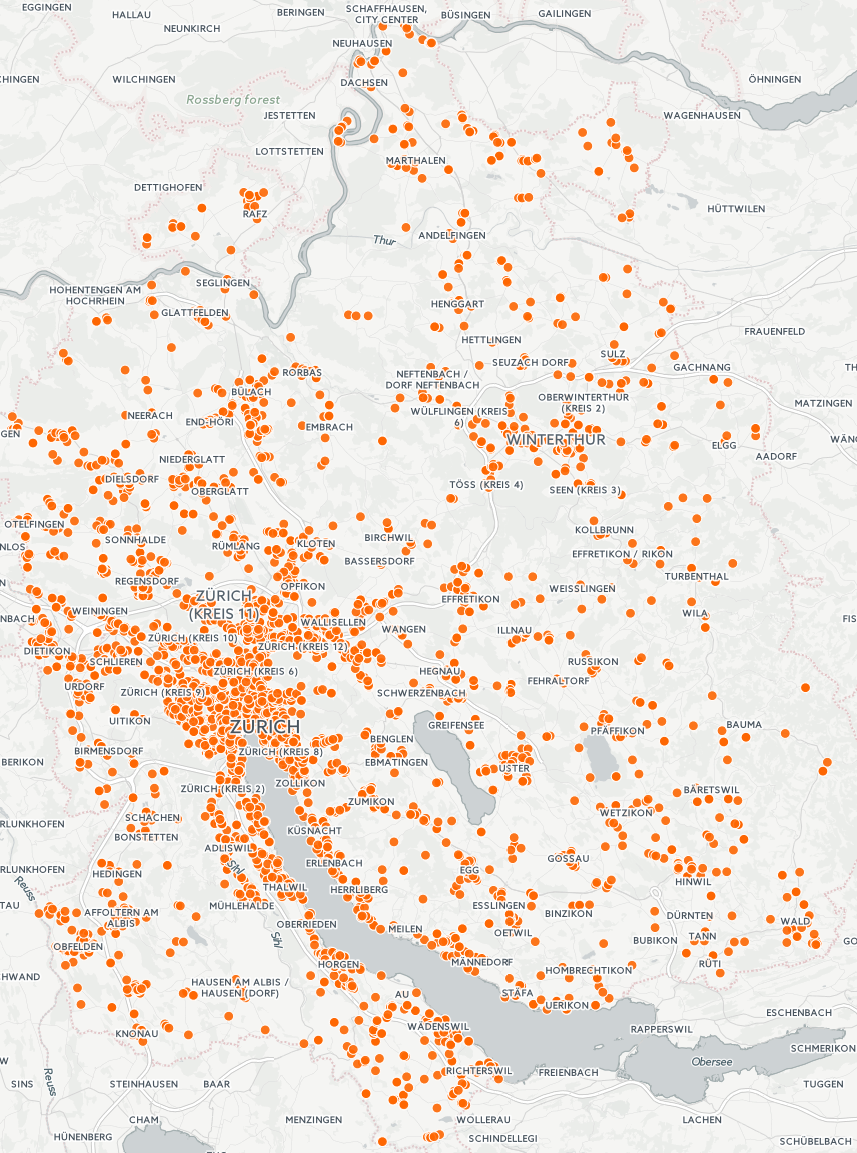
\includegraphics[width=\textwidth -80mm]{images/karte.png}
	\caption{Gesamtresultat Kanton Zürich}
\end{figure}

\subsection*{Ausblick}
Der Erkennungsalgorithmus ist zu Ende dieses Projektes auf die Region Zürich und die Ostschweiz spezialisiert. Mit weiteren Optimierungen beim Neuronalen Netz ist es möglich, alle Fussgängerstreifen in der Schweiz zu erfassen und sogar weisse Fussgängerstreifen für andere europäische Länder zu erkennen. Auch weitere Strassenmarkierungen sind denkbar.

Weiter ist die Geschwindigkeit, in der Convolutional Neural Network verbessert werden, enorm. In 2 - 3 Jahren könnte es möglich sein, annähernd alle Fussgängerstreifen auf Orthofotos zu erkennen.
\newpage